%% COSC 520 Assignment 1 - The Login Checker Problem
%% ACM Small format with the ACM, journal and copyright information removed.
%% Compile with pdfLaTeX + BibTeX (Overleaf default).

\documentclass[acmsmall,nonacm]{acmart}

\setcopyright{none}
\settopmatter{printacmref=false}
\renewcommand\footnotetextcopyrightpermission[1]{}
\pagestyle{plain}

\newcommand{\us}{\,$\mu$s}
\newcommand{\code}[1]{\texttt{#1}}

\begin{document}

\title{The Login Checker Problem: Linear Search, Binary Search, Hashing, Bloom Filters and Cuckoo Filters Compared}
\subtitle{COSC 520 Assignment 1 --- Student number 84298512}

\author{Ahmed Elgazwy}
\email{ahmed.elgazwy@ubc.ca}
\affiliation{%
  \institution{University of British Columbia}
  \city{Kelowna}
  \state{British Columbia}
  \country{Canada}}

\begin{abstract}
A sign-up service must reject a login that is already taken, and with up to a
billion users the check must be fast and small. We implement five membership
structures from scratch in Python (linear search, binary search, a chained hash
table, a Bloom filter and a cuckoo filter), derive their complexity, and
benchmark them on ten million synthetic logins, streaming the filters to one
hundred million. Lookup time grows linearly for linear search (log--log slope
1.04), logarithmically for binary search, and stays at 2--4\us{} for the hash
table and both filters. Measured false-positive rates match theory (Bloom
0.95--1.04\% against 1\%; cuckoo 0.65--0.75\% against 0.70\%). At scale memory
decides: the exact structures need 71--136 bytes per login, or 71--136\,GB for a
billion logins, while the Bloom filter needs 1.2 bytes (1.2\,GB).
\end{abstract}

\keywords{membership testing, Bloom filter, cuckoo filter, hash table, binary search, probabilistic data structures}

\maketitle

%% ---------------------------------------------------------------------------
\section{Introduction}

When a user creates an account, the service must confirm that the requested
login is not already taken. Abstractly, given a set $S$ of $n$ logins, we must
decide whether a query $x$ belongs to $S$: the \emph{membership} problem. With
millions of users, and up to $n = 10^9$ in this assignment, both the time per
query and the memory needed to answer it matter.

The textbook answers store every login exactly: a list, a sorted array or a
hash table. Bloom filters~\cite{bloom1970} and cuckoo filters~\cite{fan2014}
keep a compact, lossy summary instead. They may report a free login as taken (a
\emph{false positive}) but never a taken login as free (a \emph{false
negative}). This suits a login checker: a false positive only triggers an exact
database check or asks the user for another name, while a false negative would
create a duplicate account.

This report makes four contributions:
\begin{itemize}
  \item implementations of all five structures from scratch in Python behind one interface, with 121 unit tests;
  \item a complexity analysis, including derivations of the filters' error rates and sizes (Section~\ref{sec:complexity});
  \item a benchmark on a published synthetic dataset of $10^7$ logins, with the filters streamed to $10^8$ (Sections~\ref{sec:setup}--\ref{sec:results});
  \item a proposed alternative, the XOR filter (Section~\ref{sec:alternative}).
\end{itemize}

\noindent\textbf{Code:} \url{https://github.com/ahmedelgazwy/Advanced_DS_assignment_1}\\
\textbf{Dataset:} \url{https://github.com/ahmedelgazwy/Advanced_DS_assignment_1/releases/tag/dataset-v1}

%% ---------------------------------------------------------------------------
\section{The Five Data Structures}
\label{sec:structures}

Every structure implements \code{add(x)} and \code{contains(x)}; a sign-up
calls \code{add} only if \code{contains} says the login is free. No library
implementation is used (no \code{dict} or \code{set} as the table, no
\code{bisect}, no filter packages). Hashing uses BLAKE2b~\cite{aumasson2013} from
the standard library, which, unlike the built-in \code{hash()}, is identical on
every run, so false-positive rates are reproducible.

\textbf{Linear search} scans a list with an explicit loop (\code{x in list}
would run the scan in C and hide the cost being measured). \textbf{Binary
search} keeps the logins sorted (bulk loads use Python's Timsort) and halves the
interval to the first login not smaller than $x$. \textbf{The hash table} uses
separate chaining over $M$ slots ($M$ a power of two). Chains are created
lazily, so an empty slot costs one pointer, and $M$ doubles when the load factor
$\alpha = n/M$ exceeds 0.75.

\textbf{Bloom filter.} A bit array of $m$ bits and $k$ hash functions.
\code{add} sets bits $h_1(x), \dots, h_k(x)$. \code{contains} reports
``probably taken'' only if all $k$ bits are set. For a capacity $n$ and target
rate $p$, $m$ and $k$ follow Equations~\eqref{eq:bloom-k}--\eqref{eq:bloom-m}.
The $k$ positions come from double hashing,
$g_i(x) = h_a(x) + i\,h_b(x) \bmod m$, which has the same asymptotic error as
$k$ independent hashes~\cite{kirsch2006}, so each login is hashed once.

\textbf{Cuckoo filter.} A table of $B$ buckets with $b = 4$ slots each. Each
slot holds an $f$-bit fingerprint $\phi(x)$, and 0 marks an empty slot. A login
may live in bucket $i_1 = h(x) \bmod B$ or in $i_2 = \mathrm{alt}(i_1, \phi(x))$.
If both are full, a random resident fingerprint is evicted to its own alternate
bucket, repeating up to 500 times~\cite{fan2014}. The alternate bucket depends
only on the current bucket and the fingerprint, so fingerprints can be moved
without the original login (\emph{partial-key} cuckoo hashing, a variant of
cuckoo hashing~\cite{pagh2004}). We differ from the paper in two ways. (i) We
use $\mathrm{alt}(i, \phi) = (H(\phi) - i) \bmod B$ instead of
$i \oplus H(\phi)$: both are involutions, but ours works for any $B$, so the
table has exactly $\lceil n/(b\alpha) \rceil$ buckets instead of being rounded up
to a power of two. (ii) As in the authors' reference implementation, a
fingerprint left over when the evictions run out is kept in a one-entry victim
slot, so no stored login is lost. The table is sized for $\alpha = 0.9$; filled
until an insertion failed, it reached 96--97\% load, in line with the 95\%
reported for $b = 4$~\cite{fan2014}.

%% ---------------------------------------------------------------------------
\section{Complexity Analysis}
\label{sec:complexity}

Let $n$ be the number of stored logins and $L$ their average length ($L = 14$
in our dataset). Hashing a login costs $\Theta(L)$ and comparing two logins
costs $O(L)$. Table~\ref{tab:complexity} summarizes the results derived below.

\begin{table}[t]
\caption{Time and space complexity. $n$: logins; $L$: login length; $\alpha$: load factor; $m$, $k$: Bloom bits and hash functions; $b$, $f$: cuckoo slots per bucket and fingerprint bits. $^{*}$Expected; $^{\dagger}$amortized. The hash table's worst-case lookup is $O(nL)$; the cuckoo filter's worst-case insert is $O(L + b \cdot \mathrm{MaxKicks})$.}
\label{tab:complexity}
\small
\setlength{\tabcolsep}{5pt}
\begin{tabular}{@{}llllll@{}}
\toprule
Structure & Build & Lookup & Insert & Space & False-positive rate \\
\midrule
Linear search & $O(n)$ & $O(nL)$ & $O(1)^{\dagger}$ & $\Theta(nL)$ & 0 \\
Binary search & $O(Ln\log n)$ & $O(L\log n)$ & $O(n)$ & $\Theta(nL)$ & 0 \\
Hash table & $O(nL)^{*}$ & $O(L)^{*}$ & $O(L)^{*\dagger}$ & $\Theta(nL)$ & 0 \\
Bloom filter & $O(n(L+k))$ & $O(L+k)$ & $O(L+k)$ & $m$ bits & $(1-e^{-kn/m})^k$ \\
Cuckoo filter & $O(nL)^{*}$ & $O(L+b)$ & $O(L)^{*}$ & $nf/\alpha$ bits & $\le 2b/2^f$ \\
\bottomrule
\end{tabular}
\end{table}

\textbf{Exact structures.} Linear search makes $(n+1)/2$ comparisons on average
for a stored login and exactly $n$ for an absent one~\cite{knuth1998}. Binary
search makes at most $\lfloor \log_2 n \rfloor + 1$ comparisons (Knuth's
Algorithm~B~\cite{knuth1998}) after an $O(n \log n)$-comparison sort. Under
simple uniform hashing, a chained hash table answers a lookup in expected
$\Theta(1 + \alpha)$ time~\cite[Thms.~11.1--11.2]{cormen2022}. Doubling at
$\alpha > 0.75$ keeps $\alpha$ constant, so lookups take expected $O(1)$ time
and insertions amortized $O(1)$~\cite[\S 16.4]{cormen2022}. If every key
collides, a lookup degrades to $O(n)$. All three structures store the logins,
using $\Theta(nL)$ space. In CPython a 14-character string occupies 63 bytes,
and a list adds an 8-byte pointer, for 71 bytes per login.

\textbf{Bloom filter.} After $n$ insertions with $k$ hash functions, a given bit
is still 0 with probability $(1 - 1/m)^{kn} \approx e^{-kn/m}$. A non-member is
a false positive when all $k$ of its bits are set~\cite{broder2004,mitzenmacher2017}:
\begin{equation}
  p \approx \left(1 - e^{-kn/m}\right)^{k}.
  \label{eq:bloom-fp}
\end{equation}
This classic approximation slightly underestimates the exact rate for small
$m$~\cite{bose2008}. Minimizing Equation~\eqref{eq:bloom-fp} over $k$ gives
\begin{equation}
  k^{*} = \frac{m}{n}\ln 2, \qquad p = 2^{-k^{*}},
  \label{eq:bloom-k}
\end{equation}
so a target rate $p$ requires
\begin{equation}
  m = -\frac{n \ln p}{(\ln 2)^2} \approx 1.44\, n \log_2 \frac{1}{p}\ \text{bits.}
  \label{eq:bloom-m}
\end{equation}
For $p = 1\%$ this is 9.59 bits per login with $k = 7$. Insertion and lookup cost
$O(L + k)$. A miss stops at its first zero bit, and since about half the bits
are set at $k^{*}$, it tests at most two bits on average. The space,
$m = \Theta(n \log(1/p))$ bits, does not depend on $L$. Any structure with
false-positive rate $\varepsilon$ needs at least $n \log_2(1/\varepsilon)$
bits~\cite{carter1978}, so a Bloom filter uses 44\% more than the minimum. It
cannot delete, because clearing a bit may erase other logins.

\textbf{Cuckoo filter.} A lookup compares $\phi(x)$ with at most $2b$ stored
fingerprints, each matching by chance with probability $2^{-f}$~\cite{fan2014}:
\begin{equation}
  \varepsilon \le \frac{2b}{2^f},
  \qquad\text{so}\qquad
  f \ge \log_2 \frac{1}{\varepsilon} + \log_2 (2b).
  \label{eq:cuckoo-bound}
\end{equation}
At load factor $\alpha$ only $2b\alpha$ of those slots are occupied on average,
giving the expected rate
\begin{equation}
  \varepsilon(\alpha) \approx 1 - \left(1 - 2^{-f}\right)^{2b\alpha} \approx \frac{2b\alpha}{2^f},
  \label{eq:cuckoo-expected}
\end{equation}
which is 0.70\% for $f = 10$, $b = 4$ and $\alpha = 0.9$. The space per login is
\begin{equation}
  C = \frac{f}{\alpha} = \frac{\log_2(1/\varepsilon) + \log_2(2b)}{\alpha}\ \text{bits.}
  \label{eq:cuckoo-space}
\end{equation}
Lookup and deletion inspect two buckets, which costs $O(L + b)$. Insertion takes
$O(1)$ expected evictions while $\alpha$ stays below the maximum load, and never
more than $O(L + b \cdot \mathrm{MaxKicks})$ time. Equating
Equations~\eqref{eq:bloom-m} and~\eqref{eq:cuckoo-space} with $b = 4$ and
$\alpha = 0.95$ shows that the cuckoo filter is smaller when
$\varepsilon \lesssim 0.4\%$. Fan et al.\ report a crossover at 3\% for their
semi-sorted variant, which saves one more bit per entry.

%% ---------------------------------------------------------------------------
\section{Experimental Setup}
\label{sec:setup}

\textbf{Machine.} Intel Core i7-11800H (24\,MB L3 cache), 16\,GiB RAM,
Windows~11, Python 3.10.2. All code is single-threaded.

\textbf{Dataset.} Each login is 4--10 random lowercase letters followed by a
7-character base-36 encoding of its index, e.g.\ \code{ahftrxck0000000} (mean
length 14). The suffix makes every login unique by construction. Absent logins,
used as misses, take their indices from a disjoint range, so they can never be
stored. Generation is seeded and deterministic, and the first $n$ lines form the
dataset of size $n$. The published dataset contains $10^7$ stored logins (78\,MB
gzipped) and $10^5$ absent logins, with SHA-256 checksums.

\textbf{Choice of $n$.} The assignment suggests $n = 10^9$, but in CPython the
exact structures occupy 71--136 bytes per login (Section~\ref{sec:memory}), i.e.\
71--136\,GB at $10^9$ against 16\,GiB of RAM. We therefore benchmark all five
structures up to $n = 10^7$, where the largest (the hash table) needs 1.4\,GB.
The filters store no logins, so we also stream them to $n = 10^8$, generating
logins in chunks of $10^6$ that are discarded after insertion. At $10^9$ the
filters would fit in memory (1.2 and 2.2\,GB), but at the measured
4.6--7.1\us{} per insertion each would take 1.3--2 hours to build in pure
Python; $10^8$ already spans five orders of magnitude.

\textbf{Method.} Sizes follow 1--2--5 steps from $10^3$ to $10^7$ ($10^8$ for the
filters). Each structure is built three times per size and we report medians.
A lookup measurement uses 20{,}000 queries, half sampled from the stored logins
and half absent; linear search is capped at $2 \times 10^8$ scanned elements
(20 queries at $10^7$). The garbage collector is paused while timing, as
\code{timeit} does. Memory is the sum of \code{sys.getsizeof} over every
container and stored string, and false-positive rates use all $10^5$ absent
logins. Growth rates are the slope of a least-squares fit of
$\log(\text{time})$ against $\log n$ for $n \ge 10^4$ (1: linear, 0: constant).
The full run took 59 minutes.

%% ---------------------------------------------------------------------------
\section{Results}
\label{sec:results}

\subsection{Lookup Time}

Figure~\ref{fig:lookup} and Table~\ref{tab:results} show the three growth
classes of Table~\ref{tab:complexity}.

\textbf{Linear search is $O(n)$}: slope 1.04, 20--30\,ns per scanned element,
and 0.2\,s per lookup at $n = 10^7$. A hit costs 0.46--0.55 of a miss at every
size, matching $(n+1)/2$ versus $n$ comparisons (0.35 at $10^7$, where only 10
hits are sampled).

\textbf{The hash table and both filters take constant time}: 2--4\us{} from
$10^3$ to $10^7$ (slopes 0.08--0.11), and 3.4--4.4\us{} for the filters at
$10^8$. Most of this is interpreter overhead and hashing (one BLAKE2b call costs
about 1\us{} in Python). The small positive slopes are not extra work per
lookup; they appear once the tables outgrow the CPU cache
(Section~\ref{sec:binary}). The hash table is fastest in Python because one
hash and a chain of expected length $1 + \alpha/2$ cost less than the filters'
seven bit tests or eight slot comparisons in interpreted bytecode.

\textbf{Hits and misses differ between the filters.} A Bloom miss (2.27\us) is
faster than a hit (4.09\us) because it stops at the first zero bit. A cuckoo
miss (4.14\us) is slower than a hit (2.46\us) because it must also compute and
scan the second bucket.

\begin{figure}[t]
  \centering
  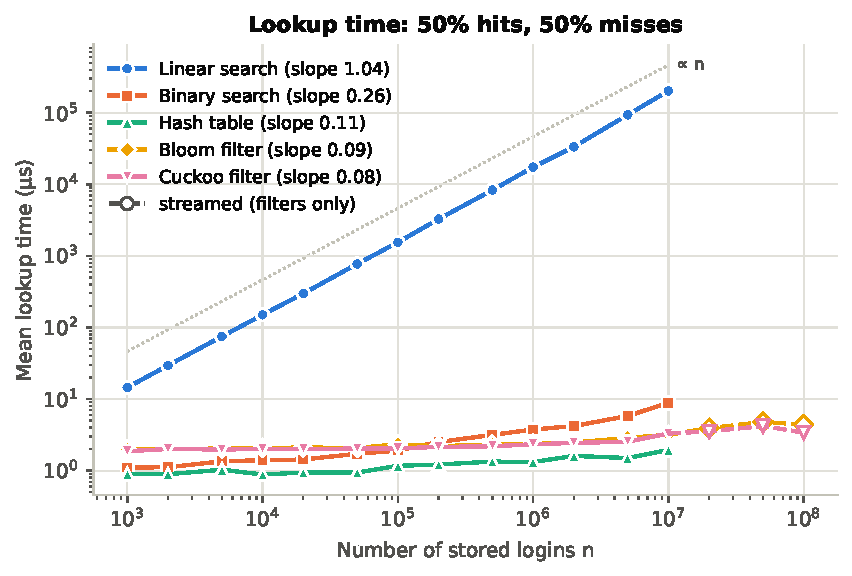
\includegraphics[width=0.85\linewidth]{figures/lookup_time.pdf}
  \caption{Mean lookup time (50\% hits, 50\% misses) against $n$ on log--log axes. Hollow markers are filters streamed beyond $10^7$. Legend slopes are fitted for $n \ge 10^4$.}
  \Description{Log-log line chart. Linear search rises from about 15 microseconds at n = 1,000 to 200,000 microseconds at 10 million, parallel to a proportional-to-n guide line. Binary search rises slowly from 1 to 9 microseconds. The hash table stays near 1 to 2 microseconds, and the Bloom and cuckoo filters near 2 to 4 microseconds up to 100 million.}
  \label{fig:lookup}
\end{figure}

\begin{table}[t]
\caption{Results at $n = 10^7$ (medians of three builds). ``Slope'' is the fitted log--log growth exponent of the lookup time.}
\label{tab:results}
\footnotesize
\setlength{\tabcolsep}{5pt}
\begin{tabular}{@{}lrrrrrr@{}}
\toprule
Structure & Build (s) & Lookup ($\mu$s) & Hit / miss ($\mu$s) & Bytes/login & FP rate & Slope \\
\midrule
Linear search & 0.09 & 201{,}725 & 104{,}671 / 298{,}779 & 71.0 & 0 & 1.04 \\
Binary search & 10.5 & 8.83 & 8.08 / 9.58 & 71.0 & 0 & 0.26 \\
Hash table & 47.9 & 1.94 & 1.82 / 2.06 & 136.0 & 0 & 0.11 \\
Bloom filter & 49.4 & 3.18 & 4.09 / 2.27 & 1.2 & 1.04\% & 0.09 \\
Cuckoo filter & 35.8 & 3.30 & 2.46 / 4.14 & 2.2 & 0.73\% & 0.08 \\
\bottomrule
\end{tabular}
\end{table}

\subsection{Binary Search and the Memory Hierarchy}
\label{sec:binary}

Binary search makes at most $\lceil \log_2(n+1) \rceil$ comparisons (10 at
$10^3$, 24 at $10^7$). While the array and its strings fit in the 24\,MB L3
cache, lookup time is linear in $\log_2 n$ at about 100\,ns per comparison
(Figure~\ref{fig:binary}). Beyond roughly $3 \times 10^5$ logins (24\,MB at 71
bytes each), probes land on uncached strings and a comparison costs up to
368\,ns. The operation count follows the analysis; only the price of an
operation changes, a hardware effect that asymptotic analysis abstracts away.

\begin{figure}[t]
  \centering
  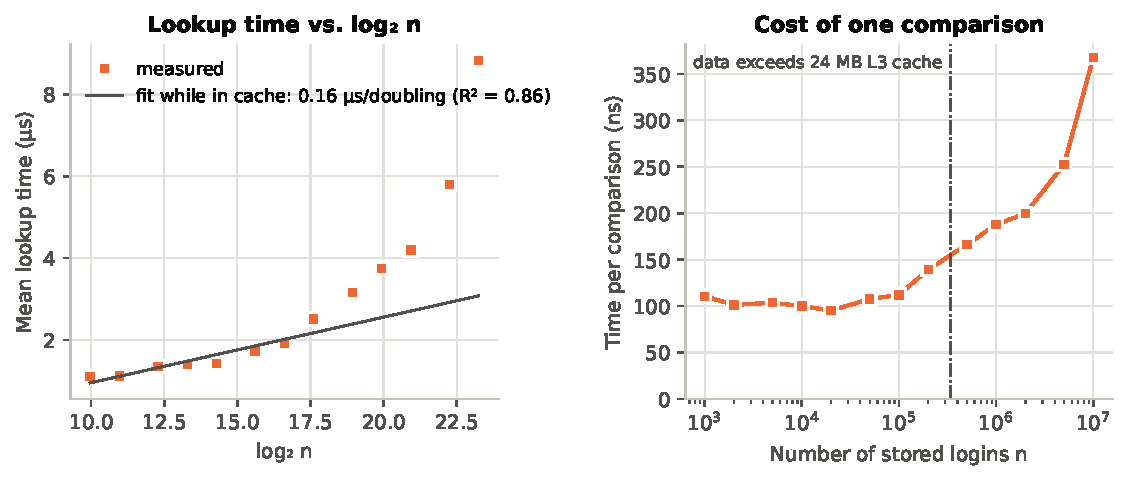
\includegraphics[width=0.95\linewidth]{figures/binary_search_log.pdf}
  \caption{Binary search. Left: lookup time against $\log_2 n$, with a linear fit over the sizes whose data fits in the L3 cache. Right: time per comparison, $t / \lceil \log_2(n+1) \rceil$, which rises once the data exceeds the 24\,MB L3 cache.}
  \Description{Two panels. Left: lookup time against log2 n rises linearly from 1.1 to about 2 microseconds up to log2 n of 17, then faster to 8.8 microseconds at log2 n of 23. Right: time per comparison is flat near 100 nanoseconds up to 100,000 logins and rises to 368 nanoseconds at 10 million; a vertical line marks where the data exceeds the 24 MB cache.}
  \label{fig:binary}
\end{figure}

\subsection{Memory}
\label{sec:memory}

Memory grows linearly for all five structures (Figure~\ref{fig:memory}).
Linear and binary search use 71 bytes per login, exactly as predicted from
CPython's object sizes, and the hash table 136--145 bytes, depending on its
load factor. The Bloom filter uses 1.20 bytes (9.59 bits) per login, as
Equation~\eqref{eq:bloom-m} predicts. The cuckoo filter uses 2.22 bytes, more
than the 11.1 bits of Equation~\eqref{eq:cuckoo-space}, because Python has no
10-bit arrays and each fingerprint occupies a 16-bit slot. Extrapolated to
$10^9$ logins, the exact structures need 71--136\,GB, several times the
machine's RAM, while the filters need 1.2\,GB (Bloom), 2.2\,GB (cuckoo as
stored) or 1.4\,GB (cuckoo, bit-packed). Memory, not time, is what rules out the
exact structures at the assignment's scale.

\begin{figure}[t]
  \centering
  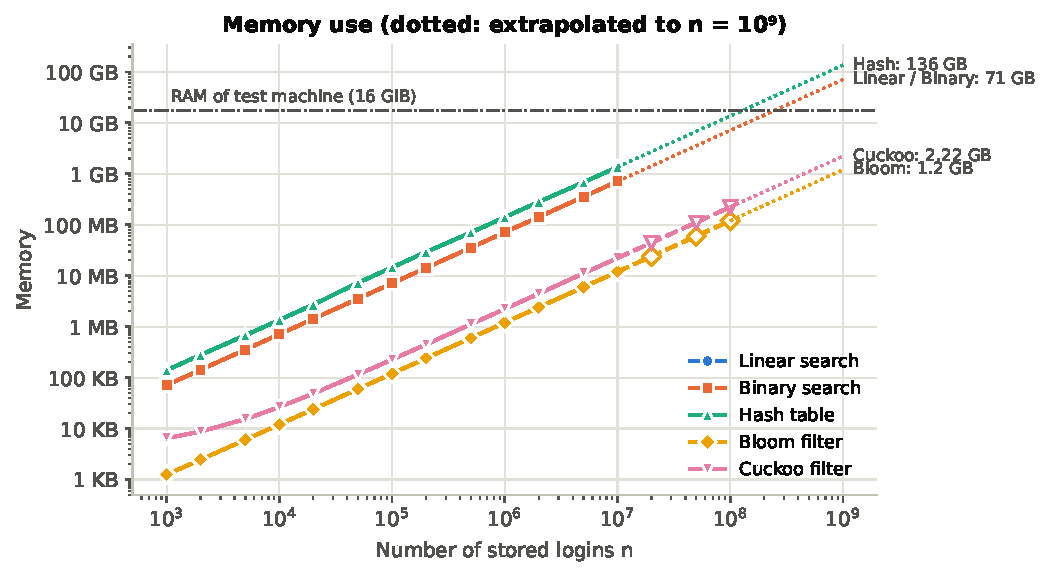
\includegraphics[width=0.85\linewidth]{figures/memory.pdf}
  \caption{Total memory against $n$. Dotted lines extrapolate the measured bytes per login to $n = 10^9$. The dash-dotted line marks the test machine's 16\,GiB of RAM.}
  \Description{Log-log chart of memory against n. The hash table, and linear and binary search, grow from about 100 kilobytes at n = 1,000 to 1.4 gigabytes and 710 megabytes at 10 million, and their extrapolations reach 136 and 71 gigabytes at one billion, above the 16 GiB RAM line. The Bloom and cuckoo filters grow from a few kilobytes to 120 and 222 megabytes at 100 million and extrapolate to 1.2 and 2.2 gigabytes.}
  \label{fig:memory}
\end{figure}

\subsection{Build Time}

All builds grow close to linearly, with slopes of 1.08--1.29
(Figure~\ref{fig:build}). The hash table and filters spend 2.5--4.9\us{} per
login at $10^6$--$10^7$, mostly hashing, and the streamed filters 7.1\us{}
(Bloom) and 4.6\us{} (cuckoo) at $10^8$. Binary search builds quickly because
Timsort runs in C, but has the highest slope (1.29), in line with
$\Theta(n \log n)$. Slopes above 1 reflect cache and allocation costs.

\begin{figure}[t]
  \centering
  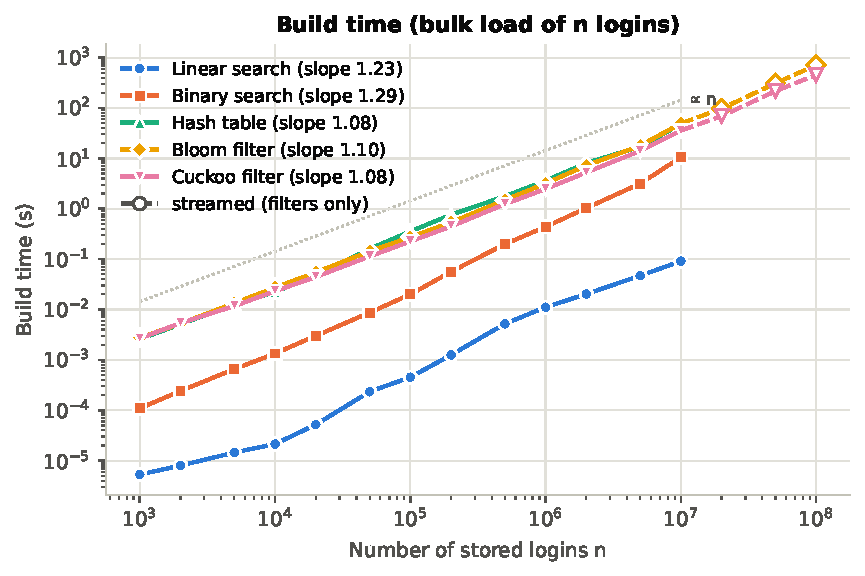
\includegraphics[width=0.72\linewidth]{figures/build_time.pdf}
  \caption{Build time for $n$ logins on log--log axes. Hollow markers are filters streamed beyond $10^7$.}
  \Description{Log-log chart. All five structures grow roughly in parallel with a proportional-to-n guide line. The hash table, Bloom and cuckoo filters take about 3 milliseconds at n = 1,000 and 36 to 49 seconds at 10 million. The filters take 455 and 713 seconds at 100 million. Binary search is about 30 times faster, and linear search about 500 times faster.}
  \label{fig:build}
\end{figure}

\subsection{False-Positive Rates}

Across 16 sizes from $10^3$ to $10^8$, the Bloom filter's measured rate stays at
0.95--1.04\%, around the 1\% of Equation~\eqref{eq:bloom-fp}
(Figure~\ref{fig:fp}). The cuckoo filter's stays at 0.65--0.75\%, around the
0.70\% expected from Equation~\eqref{eq:cuckoo-expected} and below the 0.78\%
bound of Equation~\eqref{eq:cuckoo-bound}. With $10^5$ queries the standard
error is about 0.03\%, so the spread is sampling noise. No test produced a
false negative.

\begin{figure}[t]
  \centering
  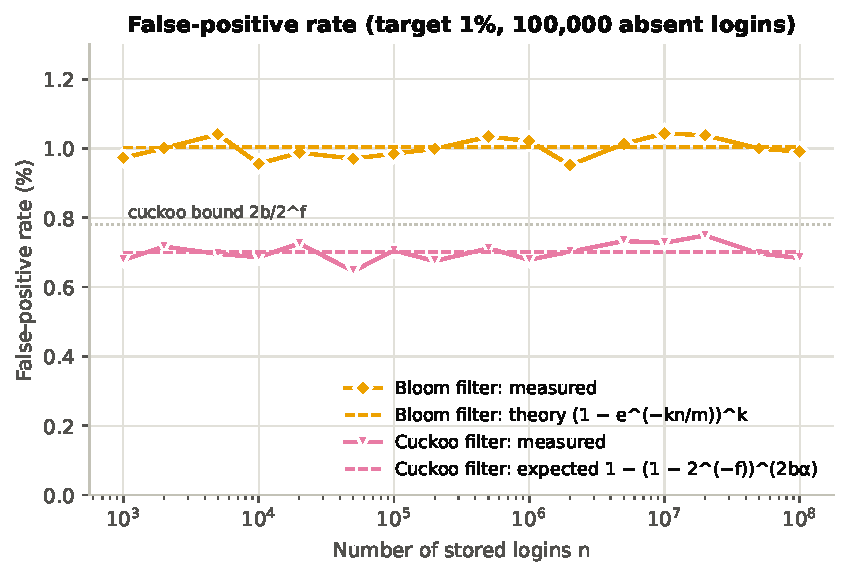
\includegraphics[width=0.72\linewidth]{figures/false_positive_rate.pdf}
  \caption{Measured false-positive rate (solid) against the theoretical value (dashed), measured on $10^5$ absent logins. The dotted line is the cuckoo filter's upper bound $2b/2^f$.}
  \Description{Line chart with n on a log axis. The Bloom filter's measured rate fluctuates between 0.95 and 1.04 percent around its flat theoretical line at 1.00 percent. The cuckoo filter's fluctuates between 0.65 and 0.75 percent around its expected 0.70 percent, below the 0.78 percent bound.}
  \label{fig:fp}
\end{figure}

\subsection{Space Versus Accuracy}

Figure~\ref{fig:tradeoff} varies the target rate from 0.1\% to 10\% at
$n = 10^6$. Counting the bits the analysis charges ($m/n$ for Bloom, $f/\alpha$
for cuckoo), the Bloom filter is smaller at loose targets and the curves cross
near 13 bits per login ($\approx$0.2\%). At the 0.1\% target, with 14.4 bits per
login each, the cuckoo filter measures 0.092\% and the Bloom filter 0.110\%,
consistent with the crossover derived in Section~\ref{sec:complexity}. As stored
in Python (8- or 16-bit slots), the cuckoo filter's points sit at 8.9 and 17.8
bits.

\begin{figure}[t]
  \centering
  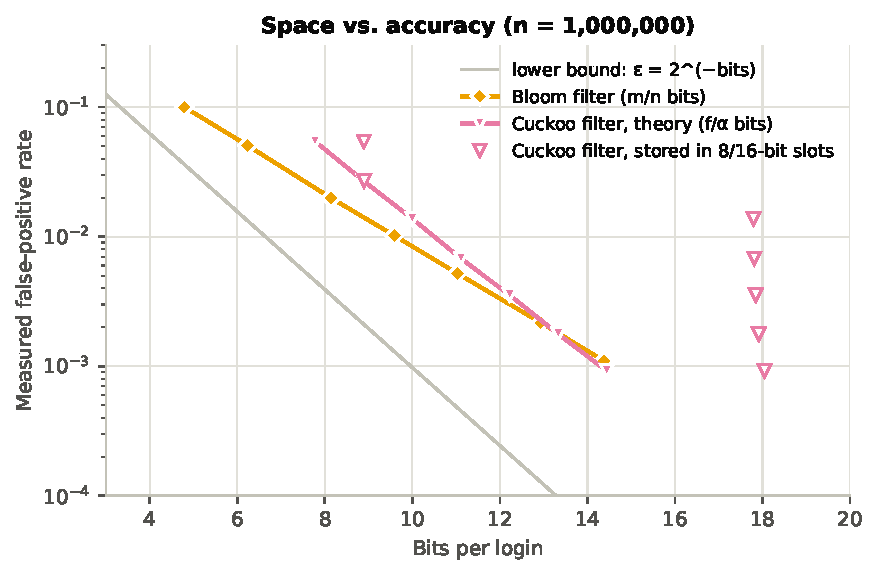
\includegraphics[width=0.72\linewidth]{figures/space_accuracy_tradeoff.pdf}
  \caption{Bits per login against the measured false-positive rate at $n = 10^6$, for targets from 0.1\% to 10\%. The gray line is the information-theoretic lower bound.}
  \Description{Log-scale chart of false-positive rate against bits per login. The Bloom filter's points lie on a straight line from 4.8 bits at 10 percent to 14.4 bits at 0.1 percent. The cuckoo filter's theoretical points start to the right of the Bloom line and cross it at about 13 bits. The cuckoo filter's stored points sit at 8.9 and 17.8 bits. All points lie above the lower-bound line.}
  \label{fig:tradeoff}
\end{figure}

%% ---------------------------------------------------------------------------
\section{Discussion}
\label{sec:discussion}

\textbf{Do the measurements support the analysis?} Yes: the growth class of
every structure (Figure~\ref{fig:lookup}), binary search's comparison count
(Figure~\ref{fig:binary}), memory per login (Figure~\ref{fig:memory}) and both
filters' error rates (Figure~\ref{fig:fp}) all match. The two deviations lie
outside the model: constant factors, which make the hash table faster than the
filters in Python, and the memory hierarchy, which raises the cost of each
operation as $n$ grows.

\textbf{Choosing a structure.} At the scale of the assignment, a filter belongs
in memory in front of the login database:
\begin{itemize}
  \item A ``definitely free'' answer, the common case during sign-up, never touches the database.
  \item A ``probably taken'' answer is confirmed by one exact lookup, which is wasted for only about 1\% of free names.
\end{itemize}
The two filters suit different needs:
\begin{itemize}
  \item \textbf{Bloom filter:} the smaller of the two at a 1\% target, the simplest, and fast on misses, but it cannot delete.
  \item \textbf{Cuckoo filter:} supports deletion (a closed account frees its name) and is smaller at very low error rates. Its lookups always touch just two buckets. However, an insertion can fail near full load, and at most $2b$ copies of one fingerprint fit.
\end{itemize}
Neither filter can grow past its planned capacity without being rebuilt from the
logins.

\textbf{Limitations.} In pure Python, interpreter overhead dominates the
constant factors; a C implementation would be much faster and would show
memory-access effects (two buckets versus $k$ scattered bits) more clearly.
Memory is counted with \code{sys.getsizeof} rather than measured by the
operating system. The logins are synthetic; real logins are skewed, but hashing
makes the filters insensitive to that. Linear search at $10^7$ used only 20
queries.

%% ---------------------------------------------------------------------------
\section{An Alternative: The XOR Filter}
\label{sec:alternative}

The XOR filter is a static membership filter that its authors report to be
both smaller and faster than Bloom and cuckoo filters~\cite{graf2020}.

\textbf{Structure.} An array $T$ of $c \approx 1.23n$ fingerprints of $f$ bits,
split into three equal blocks, and three hash functions $h_0, h_1, h_2$ that map
a key to one position in each block. The stored values satisfy, for every
$x \in S$,
\begin{equation}
  \phi(x) = T[h_0(x)] \oplus T[h_1(x)] \oplus T[h_2(x)].
\end{equation}

\textbf{Lookup.} Compute the right-hand side and compare it with $\phi(x)$.
This takes three memory accesses and no branches, so it is $O(1)$. A non-member
matches with probability $2^{-f}$.

\textbf{Construction.} The filter is built by \emph{peeling}:
\begin{enumerate}
  \item Count how many keys map to each position.
  \item Repeatedly take a position that exactly one key maps to, push that key and position on a stack, and remove the key from its other two positions. For $c \ge 1.23n$ this empties the key set with high probability; otherwise, retry with a new hash seed.
  \item Pop the stack and set each key's position so that its equation holds.
\end{enumerate}
Construction takes expected $O(n)$ time.

\textbf{Space.} $1.23 f = 1.23 \log_2(1/\varepsilon)$ bits per key, within 23\%
of the lower bound, compared with 44\% for the Bloom filter and
Equation~\eqref{eq:cuckoo-space} for the cuckoo filter. For $f = 7$
($\varepsilon \approx 0.78\%$) that is 8.6 bits per login, against 9.6 for a 1\%
Bloom filter and 11.1 for our cuckoo filter. Binary fuse filters~\cite{graf2022}
lower the overhead to about 13\% and build faster.

\textbf{Fit for login checking.} The filter is static: it cannot accept
insertions or deletions after construction. A login service could rebuild it
periodically in $O(n)$ time and keep the logins registered since the last
rebuild in a small hash table or Bloom filter that is checked alongside it.
Implementing and benchmarking this design would be the second part of the
bonus, pending the instructor's approval.

%% ---------------------------------------------------------------------------
\section{Conclusion}

All five structures answer the login checker question correctly, but only the
filters scale to the assignment's size. Linear search is $O(n)$ per lookup (0.2\,s
at ten million logins). Binary search is $O(\log n)$ but pays for cache misses.
The hash table is the fastest structure but stores every login at 136 bytes
each. The Bloom and cuckoo filters answer in 2--4\us{} up to $10^8$ logins
with 1.2--2.2 bytes per login, at a false-positive rate that matches theory
within sampling noise. For a billion users that is about 1.2\,GB instead of
more than 70\,GB.

%% ---------------------------------------------------------------------------
\section*{Use of Generative AI}

This work was produced with the assistance of Claude Code (Anthropic, Claude
Opus 5.5), an AI coding assistant, as allowed by the course policy with
disclosure. The assistant drafted the plan; generated the implementations of
the five data structures, the unit tests, and the dataset, benchmark and
plotting scripts; and drafted this report. The author directed the work phase
by phase, reviewed each phase before the next began, and chose the settings of
the experiments. Every AI-assisted source file carries the line
``AI-assisted: generated with Claude Code'' in its header.

\bibliographystyle{ACM-Reference-Format}
\bibliography{references}

\end{document}
